\chapter{Experiments}

\label{ch5_RESULTS}
\section{Dataset} 
All experiments in this project are performed on standard Hollywood2 (actions) 
\cite{hollywood2} dataset from \cite{actionsInContext}. 
It has 823 labeled training video clips and 884 labeled testing video clips. 
There are 12 activity classes : AnswerPhone, DriveCar, Eat, FightPerson,
 GetOutCar, HandShake, HugPerson, Kiss, Run, SitDown, SitUp, StandUp.
 Each clip is 10 to 30 seconds long. Frame rate is 24 fps.
 Each clip is provided with a true label. Few of the clips have multiple labels, in this project, only single labeled clips are used.


 \section{Methodology}
 \label{section_METHODOLOGY}
 {\bf Video recognizer setup - } 100,000 HoG-HoF feature vectors are randomly sampled from 
 set of all feature vectors extracted from video clips using \cite{stipCode}.
 While doing random sampling, each clip is given equal chance - this avoids biased sampling
towards (or against) any particular class of videos if they happen to be longer (or shorter) than other videos on an average.
These randomly sampled descriptors are clustered in $k = 200$ clusters using k-means.
All clips are represented in Bag-of-Features representation over these clusters as explained in section \ref{section_BOF}.

~\\
{\bf SVM - } Matlab interface of libsvm \cite{libsvm} is used to train 
12 one-vs-rest (ovr) models corresponding to 12 activity classes. A RBF kernel is used with parameters, $\gamma = 0.01$ and $C = 100$.

~\\
{\bf Object Detector Setup - } Object detector explained in section \ref{section_OBJDET} is used. 
This run of object detection has a threshold of -0.9. 
Object specific thresholding is done at a later stage while forming evidence for MLN.

The visual output of object detector looks as shown in figures \ref{fig:CarDetection} and \ref{fig:PersonDetection}. 
The boxes are called as bounding boxes.
For each box, a confidence value is also evaluated.
Table \ref{table:ObjDetection} shows sample confidence output.

\floatstyle{plain}
\restylefloat{figure}
\begin{figure}[here]
\begin{center} 
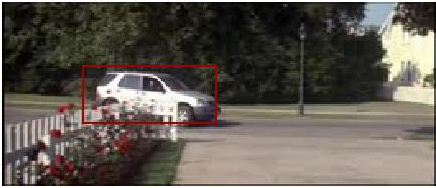
\includegraphics[scale=0.5]{car_detection_1.jpg} 
\caption[Car detection in a frame]{ Car detection in a frame. {\it Source:}\cite{hollywood2} \label{fig:CarDetection}} 
\end{center} 
\end{figure}  

\begin{figure}[here]
\begin{center} 
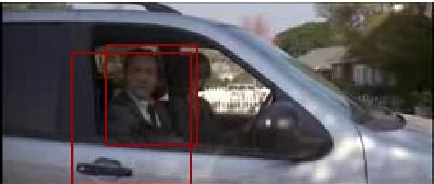
\includegraphics[scale=0.5]{person_detection_151.jpg} 
\caption[Person detection in a frame]{ Person detection in a frame. {\it Source:}\cite{hollywood2} \label{fig:PersonDetection}} 
\end{center} 
\end{figure}  

\begin{table}[t,here]
\centering
\begin{tabular}{|l|c|}
\hline
\multicolumn{2}{|c|}{FRAME1} \\
\hline
 Car            &-0.181786\\
\hline
\multicolumn{1}{|c|}\vdots & \vdots \\
\hline
\multicolumn{1}{|c|}\vdots & \vdots \\
\hline
\multicolumn{2}{|c|}{FRAME151} \\
\hline
Person	&0.579786\\
\hline
Person	&-0.593087\\
\hline
\end{tabular}
\caption{Output of object detector with decision values}
\label{table:ObjDetection}
\end{table}

Table \ref{table:ObjDetConf} shows the thresholds used to generate predicates
for evidence and inference of MLN.

\begin{table}[t,here]
\centering
\begin{tabular}{|l|c|}
\hline
Object & Threshold \\
\hline
Bicycle            &-0.90\\
\hline
Bottle            &-0.83\\
\hline
Bus            &-0.83\\
\hline
 Car            &-0.20\\
\hline
 Chair            &-0.77\\
\hline
Dining Table            &-0.80\\
\hline
Motor Bike            &-0.90\\
\hline
Person            &-0.70\\
\hline
Sofa           &-0.87\\
\hline
TV Monitor            &-0.80\\
\hline
\end{tabular}
\caption{Thresholds on object detector confidence}
\label{table:ObjDetConf}
\end{table}



~ \\
{\bf Alchemy Setup - } MLN model is learnt using Alchemy 2.0 \cite{alchemy2.0} software.
All the parameters are kept default. The learning algorithm used is the default Alchemy
learning algorithm.

~\\
{\bf Classification metric - } Predictions are compared by taking \index{Average Average Precision|see {AAP}} average average precision as a measure.
As explained in \cite{actionsInContext}, average precision(AP) approximates area under recall-precision curve.
Thus, AP for each activity class is calculated and then finally averaged over all the classes, average AP (\index{AAP}AAP) is calculated.
AP is taken as a measure of performance in the work of \cite{actionsInContext}.

\section{Results}
{\bf MLN - } Using alchemy 2.0 \cite{alchemy2.0} software, various experiments were performed 
to add the object and people information to the existing video recognizer. 
\begin{table}[t,here]
\centering
\captionsetup{justification=centering,margin=2cm}
\begin{tabular}{| l | c | c | c | c |}
\hline
	{\bf Activity Class} 
	&\multicolumn{4}{c|}{\centering {\bf MLN} }\\ \hline

	~ 
	& \multicolumn{1}{p{1.2cm}|}{\centering {\bf Only \\ Action}}
	& \multicolumn{1}{p{1.2cm}|}{\centering {\bf Action \& \\ Object}}
	& \multicolumn{1}{p{1.2cm}|}{\centering {\bf Action \& \\ People}}
	& \multicolumn{1}{p{1.2cm}|}{\centering {\bf Action \\ Object \& \\ People}}
	\\ \hline
	AnswerPhone	& 10.64\%  & 11.11\%  & 11.67\%  & 12.73\%  \\ \hline
	DriveCar  	& 66.06\%  & 66.67\%  & 71.57\%  & 68.18\%  \\ \hline
	Eat  		& 32.50\%  & 40.00\%  & 35.00\%  & 40.00\%  \\ \hline
	FightPerson  	& 56.90\%  & 54.84\%  & 61.54\%  & 62.26\%  \\ \hline
	GetOutCar  	& 8.00\%   & 13.79\%  & 17.39\%  & 14.29\%  \\ \hline
	HandShake  	& 21.43\%  & 25.00\%  & 30.77\%  & 41.67\%  \\ \hline
	HugPerson  	& 15.79\%  & 13.79\%  & 14.29\%  & 16.13\%  \\ \hline
	Kiss  		& 18.07\%  & 19.78\%  & 19.79\%  & 20.65\%  \\ \hline
	Run  		& 36.42\%  & 41.48\%  & 40.32\%  & 42.15\%  \\ \hline
	SitDown  	& 38.10\%  & 35.56\%  & 34.78\%  & 39.56\%  \\ \hline
	SitUp  		& 0.00\%   & 5.26\%   & 0.00\%   & 12.50\%  \\ \hline
	StandUp  	& 38.46\%  & 36.29\%  & 38.26\%  & 36.24\%  \\ \hline
	AAP  		& 28.53\%  & 30.30\%  & 31.28\%  & 33.86\%  \\ \hline

\end{tabular}
\caption{MLN Experiments - Average precisions}
\label{table:MLN_RESULTS}
\end{table}


\begin{comment}
\begin{table}[t,here]
\centering
\captionsetup{justification=centering,margin=2cm}
\begin{tabular}{| l | c | c | c | c | c |}
\hline
	{\bf Activity Class} & {\centering {\bf SVM}}
	&\multicolumn{4}{c|}{\centering {\bf MLN} }\\ \hline

	~ & ~
	& \multicolumn{1}{p{1.2cm}|}{\centering {\bf Only \\ Action}}
	& \multicolumn{1}{p{1.2cm}|}{\centering {\bf Action \& \\ Object}}
	& \multicolumn{1}{p{1.2cm}|}{\centering {\bf Action \& \\ People}}
	& \multicolumn{1}{p{1.2cm}|}{\centering {\bf Action \\ Object \& \\ People}}
	\\ \hline
	AnswerPhone	& 11.36\%  & 10.64\%  & 11.11\%  & 11.67\%  & 12.73\%  \\ \hline
	DriveCar  	& 66.96\%  & 66.06\%  & 66.67\%  & 71.57\%  & 68.18\%  \\ \hline
	Eat  		& 45.45\%  & 32.50\%  & 40.00\%  & 35.00\%  & 40.00\%  \\ \hline
	FightPerson  	& 57.63\%  & 56.90\%  & 54.84\%  & 61.54\%  & 62.26\%  \\ \hline
	GetOutCar  	& 17.86\%  & 8.00\%   & 13.79\%  & 17.39\%  & 14.29\%  \\ \hline
	HandShake  	& 25.93\%  & 21.43\%  & 25.00\%  & 30.77\%  & 41.67\%  \\ \hline
	HugPerson  	& 15.15\%  & 15.79\%  & 13.79\%  & 14.29\%  & 16.13\%  \\ \hline
	Kiss  		& 18.18\%  & 18.07\%  & 19.78\%  & 19.79\%  & 20.65\%  \\ \hline
	Run  		& 38.78\%  & 36.42\%  & 41.48\%  & 40.32\%  & 42.15\%  \\ \hline
	SitDown  	& 40.96\%  & 38.10\%  & 35.56\%  & 34.78\%  & 39.56\%  \\ \hline
	SitUp  		& 5.26\%   & 0.00\%   & 5.26\%   & 0.00\%   & 12.50\%  \\ \hline
	StandUp  	& 35.20\%  & 38.46\%  & 36.29\%  & 38.26\%  & 36.24\%  \\ \hline
	AAP  		& 31.56\%  & 28.53\%  & 30.30\%  & 31.28\%  & 33.86\%  \\ \hline

\end{tabular}
\caption{MLN Experiments - Average precisions}
\label{table:MLN_RESULTS}
\end{table}
\end{comment}

Table \ref{table:MLN_RESULTS} shows comparison of APs for various strategies using MLNs.
As can be seen, Average AP, when only action is considered for evidence and inference, is 28.53\%. 
This number gradually improves as more information is brought into the system.
Action information when added with Object information shows Average AP to be 30.30\%. 
Action and People information shows Average AP to be 31.28\%.
And finally, adding both Object and People information to action information,
Average AP of 33.86\% is achieved.


~\\

{\bf Object and People Features in SVM - }
The Bag-of-Features vector of each clip can be appended with Object and People features.
Term Frequency - Inverse Document Frequency (tf-idf) counts of objects are taken as object features.
One feature corresponding to one object.
Average number of people per frame are taken as people features.
Thus adding 11 more features to each feature vector.
These new feature vectors are now used to learn SVM model with similar parameters 
and methodology explained in section \ref{section_METHODOLOGY}.
It shows significant improvement as described in table \ref{table:SVM_TFIDF}.


\begin{table}[t,here]
\centering
\captionsetup{justification=centering,margin=2cm}
\begin{tabular}{| l | c | c | c | c |}
\hline
	{\bf Activity Class}
	& \multicolumn{1}{p{2cm}|}{\centering {\bf SVM Basic}}
	& \multicolumn{1}{p{2cm}|}{\centering {\bf SVM Basic\\ + Object} }
	& \multicolumn{1}{p{2cm}|}{\centering {\bf SVM Basic\\ + People} }
	& \multicolumn{1}{p{2cm}|}{\centering {\bf SVM Basic\\ + People \\+ Object} } \\ \hline
AnswerPhone & 11.36\% & 11.63\% & 16.67\% & 16.67\% \\ \hline
DriveCar & 66.96\%  & 66.69\% & 70.09\% & 70.09\% \\ \hline
Eat & 45.45\% & 44.12\% & 35.00\% & 50.00\% \\ \hline
FightPerson & 57.63\%  & 57.63\% & 60.00\% & 66.04\% \\ \hline
GetOutCar & 17.86\%  & 17.86\% & 10.34\% & 12.12\% \\ \hline
HandShake & 25.93\%  & 25.93\% & 36.36\% & 31.82\% \\ \hline
HugPerson & 15.15\%  & 15.62\% & 17.86\% & 17.86\% \\ \hline
Kiss & 18.18\%  & 18.18\% & 17.65\% & 20.69\% \\ \hline
Run & 38.78\%  & 38.51\% & 36.42\% & 39.35\% \\ \hline
SitDown & 40.96\%  & 40.96\% & 42.68\% & 42.05\% \\ \hline
SitUp & 5.26\%  & 5.26\% & 4.55\% & 8.70\% \\ \hline
StandUp & 35.20\%  & 35.20\% & 37.21\% & 37.88\%\\ \hline
Average AP & 31.56\%  & 31.49\% & 31.64\% & 34.44\% \\ \hline
%
\end{tabular}
\caption{Average Precision : Object and People Features in SVM}
\label{table:SVM_TFIDF}
\end{table}



\begin{comment}
\begin{table}[t,here]
\centering
\captionsetup{justification=centering,margin=2cm}
\begin{tabular}{| l | c | c |}
\hline
	{\bf Activity Class}
	& \multicolumn{1}{p{3cm}|}{\centering {\bf AP - Basic \\ SVM}}
	& \multicolumn{1}{p{3cm}|}{\centering {\bf AP - Object \\ and People} }\\ \hline
AnswerPhone & 11.36\% & 16.67\% \\ \hline
DriveCar & 66.96\% & 70.09\% \\ \hline
Eat & 45.45\% & 50.00\% \\ \hline
FightPerson & 57.63\% & 66.04\% \\ \hline
GetOutCar & 17.86\% & 12.12\% \\ \hline
HandShake & 25.93\% & 31.82\% \\ \hline
HugPerson & 15.15\% & 17.86\% \\ \hline
Kiss & 18.18\% & 20.69\% \\ \hline
Run & 38.78\% & 39.35\% \\ \hline
SitDown & 40.96\% & 42.05\% \\ \hline
SitUp & 5.26\% & 8.70\% \\ \hline
StandUp & 35.20\% & 37.88\%\\ \hline
Average AP & 31.56\% & 34.44\% \\ \hline
%
\end{tabular}
\caption{Average Precision : Object and People Features in SVM}
\label{table:SVM_TFIDF}
\end{table}
\end{comment}

Advantage of {\bf MLN approach over SVM} approach is that, MLNs can support feed-backs.
A high confidence of an activity can increase probability of object being present in that particular clip. 
This kind of feedback information cannot be captured using Object and People SVM features.

